\documentclass[12pt,a4paper,oneside, titlepage]{report}

\usepackage[utf8]{inputenc}
\usepackage[T1]{fontenc}
\usepackage[french]{babel}
\usepackage{amssymb}
\usepackage{amsmath}
\usepackage{graphicx}
\usepackage{float}
\usepackage{mathtools}


\author{Matteo Besançon}

\title {Parallélisme \\ \large TP 4}
\date{\today}


\begin{document}

	\maketitle
	\newpage

	\section*{Introduction}
	Dans ce TP on cherche à modéliser la propagation de chaleur sur une plaque métalique rectangulaire dont deux bords sont soumis à une contrainte de chaleur.

	Pour cela nous utilisons l'équation différentielle suivante :

	$$\frac{\delta u}{\delta t} = \alpha (\frac{\delta^2 u}{\delta x^2} + \frac{\delta^2 u}{\delta y^2})$$

	Avec l'équation de Laplace on arrive au dévelopement suivant :

	$$u(i, j)^{k+1}=\frac{1}{4}(u(i+1, j)^{(k)}+ u(i-1, j)^{(k)} + u(i, j+1)^{(k)} + u(i, j-1)^{(k)})$$

	Avec un grand nombre d'itération, il est possible d'aproximer la répartition de chaleur sur la plaque métalique.

	Cepedant, suivant le niveau de résolution souhaité (taille de la matrice représentant la plaque), cet façon de faire est très couteuse en puissance de calcule.
	De ce fait, il devient très intéressant de paralléliser cet algorithme. Pour cela on divise la matrice en sous-matrice afin de répartire les calcules sur plusieurs CPU.

	Dans notre cas, nous avons divisé la matrice en bandes comprenant entre une et plusieurs lignes de la matrice.
	Il nous est donc nécessaire d'avoir une communication entre les différents CPU pour gérer les valeurs nécesaire pour le calcul du bord inférieur et supérieur du sous-domaine.

	\section*{Méthode}

	Pour obtenir mes résultats, je me suis basé sur le code que j'ai élaboré au TP2 en y ajoutant des mesures de temps.
	Ces mesures on été effectuées à plusieurs endroit du code afin d'optenir les temps suivants :

	\begin{itemize}
		\item Temps d'execution total de l'algorithme
		\item Temps d'execution de la boucle principale (execution du calcul de répartition de chaleur)
		\item Temps d'écriture de la matrice finale sur le disque
	\end{itemize}

	Les mesures ont étés effectuées sur baobab en utilisant 1, 2, 10, 20, 40, 60, 80, 100 et 120 processeurs pour des matrices carrées ayant un bord de 2000, 3000 et 4000.
	Le nombre d'itération a lui été fixé à 3000 de façon à obtenir des temps d'exécutions compris entre environ 16 et 5900 secondes.

	Comme expliqué dans la donnée, il est ensuite possible de calculer $\alpha$ constante représentant le temps de calcule et $\beta$ représentant le temps de communication par régression linéaire.
	Pour cela on se base sur la formule suivante

	$$T_{par} = \alpha \frac{N^2}{p}+ \beta N$$

	où $N$ est la taille de la matrice et $p$ le nombre de processeurs.

	Avec les résultats obtenus il est également possible de calculer le speedup ($S$) représentant le gain de temps de notre algorithme.
	Il peut peut être calculé comme cela

	$$S = \frac{T_{seq}}{T_{par}}$$

	Le speedup peut également être calculé avec la loi de Amdahl qui nous permet d'obtenir

	$$S = \frac{1}{\gamma + \frac{1 - \gamma}{p}}$$

	$\gamma$ étant la partie non-parallélisable d'un algorithme.

	Il nous est possible d'aproximer $\gamma$ à partire de nos résultats.
	Pour cela, j'ai décidé de procéder de deux façons différentes.
	La première étant de se baser sur le temps d'exécutions total de notre algorithme et le temps d'exécutions de la boucle principale.
	Dans ce cas on a la relation suivante

	$$\gamma = 1- \frac{T_{loop}}{T_{tot}}$$

	La deuxième façon est de se baser sur le temps d'execution de la boucle principale et le temps d'écriture sur le disque.
	Da ce cas on a

	$$\gamma = 1- \frac{T_{loop}}{T_{loop} + T_{write}}$$

	\newpage

	\section*{Résultats}

	Pour le temps d'exécution on obtien les résultats suivants.

	\begin{table}[H]
\begin{tabular}{lc|l|l|l|}
\cline{3-5}
                      & \multicolumn{1}{l|}{} & \multicolumn{3}{c|}{\textbf{Matrix size}}                                                                    \\ \cline{2-5}
\multicolumn{1}{l|}{} & \textbf{CPU nb}       & \multicolumn{1}{c|}{\textbf{2000}} & \multicolumn{1}{c|}{\textbf{3000}} & \multicolumn{1}{c|}{\textbf{4000}} \\ \cline{2-5}
\multicolumn{1}{l|}{} & \textbf{1}            & 1493.28                            & 3353.38                            & 5828.97                            \\ \cline{2-5}
\multicolumn{1}{l|}{} & \textbf{2}            & 720.996                            & 1631.92                            & 2669.38                            \\ \cline{2-5}
\multicolumn{1}{l|}{} & \textbf{10}           & 130.063                            & 302.791                            & 602.044                            \\ \cline{2-5}
\multicolumn{1}{l|}{} & \textbf{20}           & 74.2869                            & 173.232                            & 304.306                            \\ \cline{2-5}
\multicolumn{1}{l|}{} & \textbf{40}           & 39.5911                            & 92.0058                            & 162.637                            \\ \cline{2-5}
\multicolumn{1}{l|}{} & \textbf{60}           & 29.4361                            & 63.2842                            & 112.878                            \\ \cline{2-5}
\multicolumn{1}{l|}{} & \textbf{80}           & 22.4701                            & 49.5435                            & 89.8998                            \\ \cline{2-5}
\multicolumn{1}{l|}{} & \textbf{100}          & 19.0033                            & 41.6588                            & 73.7928                            \\ \cline{2-5}
\multicolumn{1}{l|}{} & \textbf{120}          & 16.6479                            & 36.5544                            & 60.3538                            \\ \cline{2-5}
\end{tabular}
\caption{Temps d'exécution total de l'algoritme [s]}
\end{table}

\begin{table}[H]
\begin{tabular}{lc|l|l|l|}
\cline{3-5}
                      & \multicolumn{1}{l|}{} & \multicolumn{3}{c|}{\textbf{Matrix size}}                                                                    \\ \cline{2-5}
\multicolumn{1}{l|}{} & \textbf{CPU nb}       & \multicolumn{1}{c|}{\textbf{2000}} & \multicolumn{1}{c|}{\textbf{3000}} & \multicolumn{1}{c|}{\textbf{4000}} \\ \cline{2-5}
\multicolumn{1}{l|}{} & \textbf{1}            & 1490.55                            & 3347.53                            & 5818.64                            \\ \cline{2-5}
\multicolumn{1}{l|}{} & \textbf{2}            & 718.364                            & 1625.79                            & 2661.95                            \\ \cline{2-5}
\multicolumn{1}{l|}{} & \textbf{10}           & 127.692                            & 297.738                            & 593.096                            \\ \cline{2-5}
\multicolumn{1}{l|}{} & \textbf{20}           & 71.806                             & 167.581                            & 295.432                            \\ \cline{2-5}
\multicolumn{1}{l|}{} & \textbf{40}           & 36.8802                            & 86.253                             & 152.95                             \\ \cline{2-5}
\multicolumn{1}{l|}{} & \textbf{60}           & 26.413                             & 57.1772                            & 103.96                             \\ \cline{2-5}
\multicolumn{1}{l|}{} & \textbf{80}           & 19.5576                            & 43.697                             & 80.3897                            \\ \cline{2-5}
\multicolumn{1}{l|}{} & \textbf{100}          & 16.0662                            & 35.3686                            & 64.2113                            \\ \cline{2-5}
\multicolumn{1}{l|}{} & \textbf{120}          & 13.6203                            & 30.541                             & 51.3374                            \\ \cline{2-5}
\end{tabular}
\caption{Temps d'exécution de la boucle principale [s]}
\end{table}

\begin{table}[H]
\begin{tabular}{lc|l|l|l|}
\cline{3-5}
                      & \multicolumn{1}{l|}{} & \multicolumn{3}{c|}{\textbf{Matrix size}}                                                                    \\ \cline{2-5}
\multicolumn{1}{l|}{} & \textbf{CPU nb}       & \multicolumn{1}{c|}{\textbf{2000}} & \multicolumn{1}{c|}{\textbf{3000}} & \multicolumn{1}{c|}{\textbf{4000}} \\ \cline{2-5}
\multicolumn{1}{l|}{} & \textbf{1}            & 2.41715                            & 5.14431                            & 9.02354                            \\ \cline{2-5}
\multicolumn{1}{l|}{} & \textbf{2}            & 2.46384                            & 5.74968                            & 6.70621                            \\ \cline{2-5}
\multicolumn{1}{l|}{} & \textbf{10}           & 2.30698                            & 4.91582                            & 8.65097                            \\ \cline{2-5}
\multicolumn{1}{l|}{} & \textbf{20}           & 2.41974                            & 5.5249                             & 8.65585                            \\ \cline{2-5}
\multicolumn{1}{l|}{} & \textbf{40}           & 2.59763                            & 5.38511                            & 9.30727                            \\ \cline{2-5}
\multicolumn{1}{l|}{} & \textbf{60}           & 2.64123                            & 5.67702                            & 8.64367                            \\ \cline{2-5}
\multicolumn{1}{l|}{} & \textbf{80}           & 2.63721                            & 5.57048                            & 9.03595                            \\ \cline{2-5}
\multicolumn{1}{l|}{} & \textbf{100}          & 2.61988                            & 5.86432                            & 9.04519                            \\ \cline{2-5}
\multicolumn{1}{l|}{} & \textbf{120}          & 2.64166                            & 5.54288                            & 8.64299                            \\ \cline{2-5}
\end{tabular}
\caption{Temps d'écriture sur le disque [s]}
\end{table}

On compile les données dans le graph suivant

	\begin{figure}[H]
		\caption {Temps d'exécution avec droites de régression}
    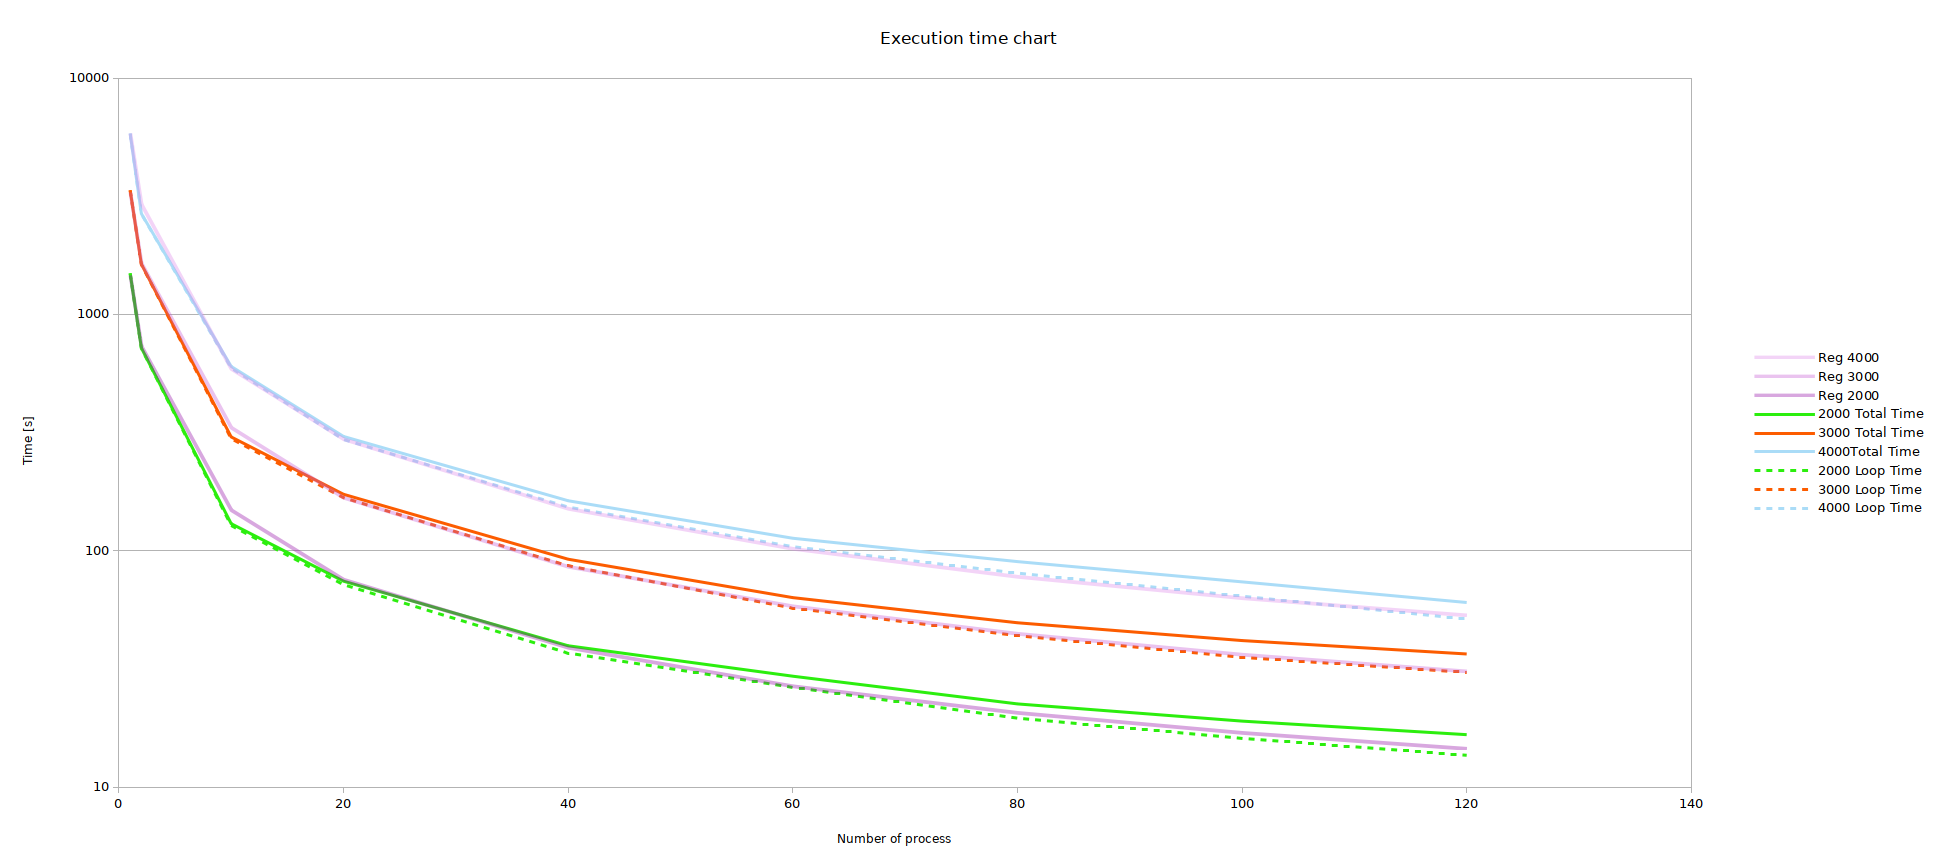
\includegraphics[scale=0.32]{time}
    \centering
  \end{figure}

	Les mesures effectuées nous on permis de calculer les valeurs suivantes pour $\alpha$ et $\beta$

	$$\alpha = 0.000363318027893$$
	$$\beta = 0.001163137873659$$

	\newpage

	Pour ce qui est du speedup, nous avons calculé les $\gamma$ suivants

	$$\gamma = 1- \frac{T_{loop}}{T_{tot}} = 0.001781627184593$$
	$$\gamma = 1- \frac{T_{loop}}{T_{loop} + T_{write}} = 0.001567270604976$$

	On a donc le graph de speedup suivant

	\begin{figure}[H]
		\caption {Speedup effectif et théorique du programme}
		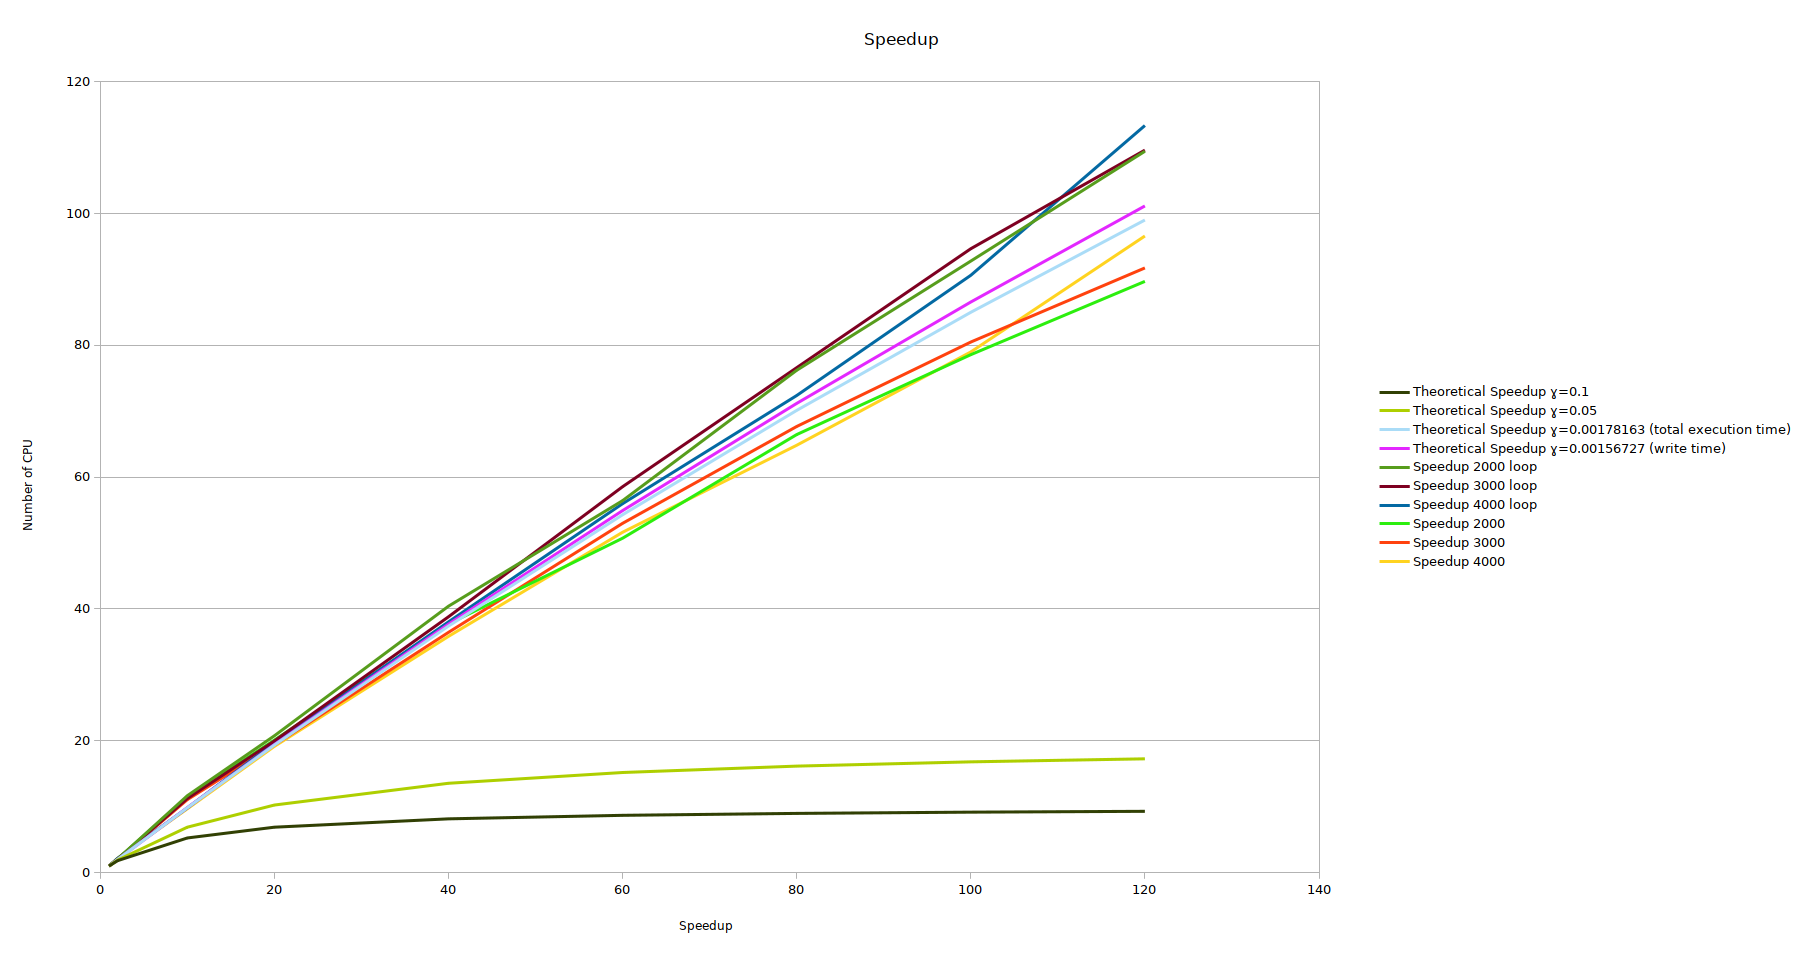
\includegraphics[scale=0.32]{speedup}
		\centering
	\end{figure}

	\section*{Conclusion}

	On peut voir dans les résultats obtenus que le Speedup obtenu par cet algorithme est très important.
	Il est donc très intéressant de paralléliser l'execution de ce progamme dans un souci de performance.

	On voit que les résults obtenus somblent cohérents car le speedup obtenu pour la boucle principale plus grand que celui de l'algorithme entier.
	En effet, en concidérent l'algoritme dans son ensemble, les parties d'organisation des cpu, de communication et d'écriture sur le disque sont des parties non-parallélisable.

	On voit également  que le speedup de la boucle principale est proche du speedup optimal (partie non-parallélisable nul).
	On peut donc en déduire que, lorsque la communication inter CPU est gérée de façon efficace, la perte d'efficacité est moindre.

	Pour finir, on peut voire que la partie non parallélisable estimée à l'aide des deux méthodes décrites précédement est relativement fiable.
	On obtient un speedup théorique légèrement supérieur à celui mesuré sur la totalité de l'algorithme et inférieur à celui de la boucle principale.
	Le fait que ce speedup théorique est légèrement plus élevé que celui obtenu dans la réalité peut être expoliqué simplement par le fait que nous avons uniquement pris en compte le temps d'écriture sur le disque ainsi que la temps de communication intern à la boucle pricipal, sans tenir compte de la comunication et la mise en place initial.
	En effet cette partie étant non-parallélisable, elle diminue le speedup effectif de l'algoritme.


\end{document}
